\documentclass[conference]{IEEEtran}
\IEEEoverridecommandlockouts

\usepackage{cite}
\usepackage{amsmath,amssymb,amsfonts}
\usepackage{graphicx}
\usepackage{enumitem}
\usepackage{makecell}
\usepackage{textcomp}
\usepackage{listings}
\usepackage{xcolor}
\usepackage{hyperref}

\def\BibTeX{{\rm B\kern-.05em{\sc i\kern-.025em b}\kern-.08em
    T\kern-.1667em\lower.7ex\hbox{E}\kern-.125emX}}

\begin{document}
%\begin{flushleft}
 %   
\includegraphics[width=6.5cm]{IIITB-COMET-Logo.png}
%\end{flushleft}
\title{Voice‑Controlled Obstacle‑Avoiding UGV Using ESP32}
\author{
    \IEEEauthorblockN{Srinivas Namathoti}
      \textbf{Instructor: S. Srikanth Reddy}
    \IEEEauthorblockA{
    Future Wireless Cmmunnications 5G/6G\\
             IIITB COMET, Bangalore, India \\
    Email: \texttt{srinivas.fwc@iiitb.ac.in}
    }
}

\maketitle


\begin{abstract}
This paper presents a voice‑controlled unmanned ground vehicle (UGV) built using an ESP32 microcontroller and an L298N motor driver. The UGV is controlled via voice commands using a Bluetooth‑connected Android application. An ultrasonic sensor is integrated to detect and avoid obstacles in the path; a buzzer provides alerts when an obstacle is detected. This low‑cost and scalable platform serves as a prototype for intelligent robotics systems with human–robot voice interaction and autonomous navigation.
\end{abstract}

\section{Introduction}
Voice‑based human‑robot interaction offers an intuitive control method for robotic platforms. In recent years, voice recognition integrated with embedded systems has enabled robots to respond to spoken commands and perform autonomous tasks. In this project, we demonstrate a voice‑controlled UGV prototype using the ESP32 microcontroller and the L298N motor driver. The system is enhanced with an ultrasonic sensor for obstacle detection and a buzzer for user alerting when obstacles are detected.

\section{Hardware Setup}
The components used in this project are listed in Table~\ref{table:components}.

\begin{table}[!ht]
\centering
\caption{List of Components}
\label{table:components}
\begin{tabular}{|c|l|}
\hline
\textbf{S.No} & \textbf{Component} \\
\hline
1 & ESP32 Development Board \\
2 & L298N Motor Driver Module \\
3 & DC Motors (2×) \\
4 & Toy Car Chassis with Wheels \\
5 & Breadboard \\
6 & Connecting Wires \\
7 & Ultrasonic Sensor (HC‑SR04) \\
8 & Buzzer Module \\
9 & Power Bank with USB Cable \\
\hline
\end{tabular}
\end{table}

\subsection{Motor Connections (ESP32 to L298N)}
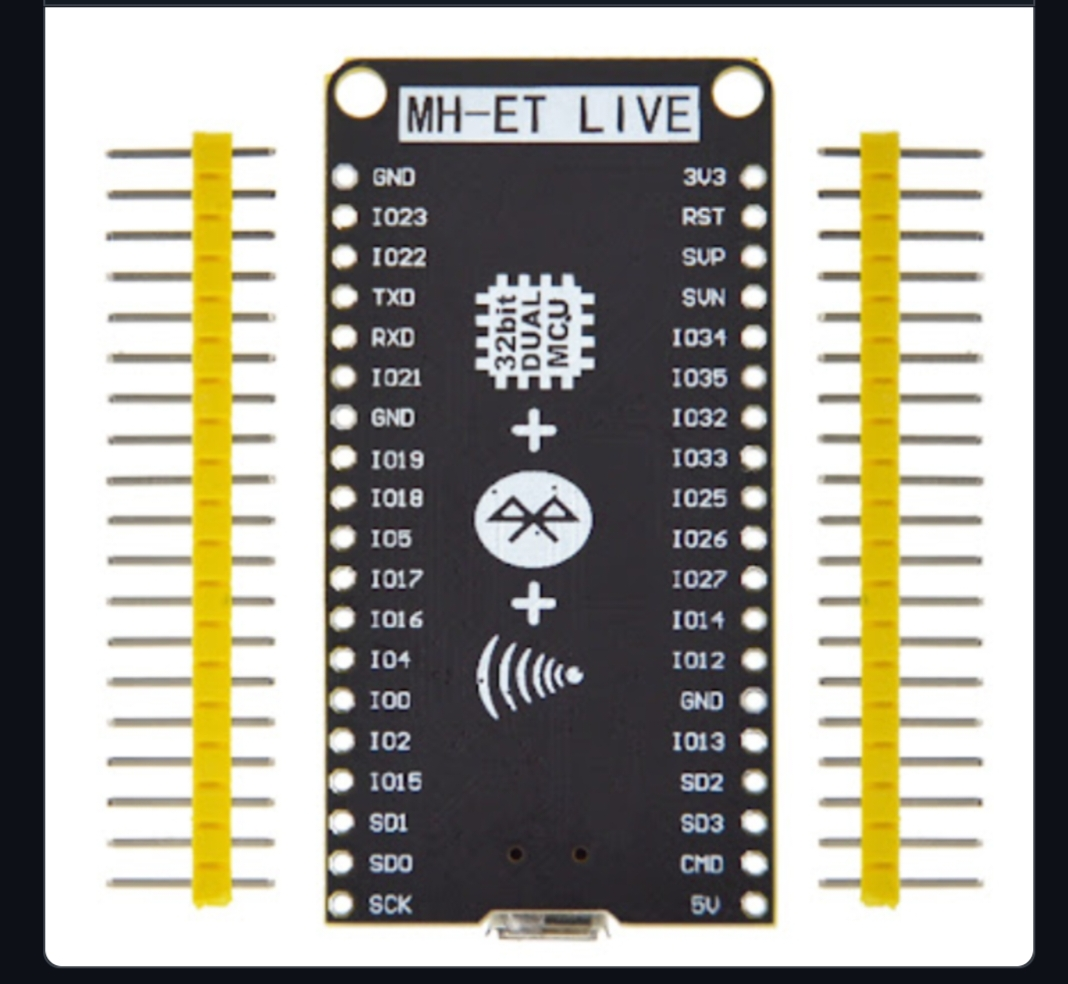
\includegraphics[width=0.4\linewidth]{esp32.jpg}
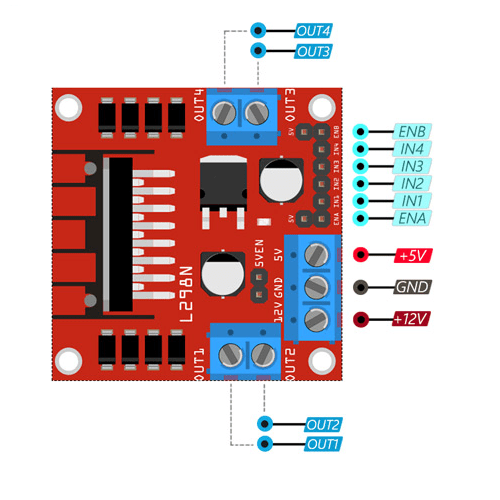
\includegraphics[width=0.4\linewidth]{L298N.png}
\begin{table}[!ht]
\centering
\caption{ESP32 to L298N Motor Driver Connections}
\begin{tabular}{|c|c|c|}
\hline
\textbf{ESP32 Pin} & \textbf{L298N Pin} & \textbf{Description} \\
\hline
GPIO 23 & IN1 & Motor A direction control \\
GPIO 22 & IN2 & Motor A direction control \\
GPIO 21 & IN3 & Motor B direction control \\
GPIO 19 & IN4 & Motor B direction control \\
5V       & VCC & Power supply to driver \\
GND      & GND & Common ground \\
\hline
\end{tabular}
\end{table}

\subsection{Ultrasonic Sensor Connections (HC‑SR04)}
\begin{table}[!ht]
\centering
\caption{Ultrasonic Sensor to ESP32 Connections}
\begin{tabular}{|c|c|}
\hline
\textbf{HC‑SR04 Pin} & \textbf{ESP32 Pin} \\
\hline
VCC & 5V \\
GND & GND \\
Trig & GPIO 2 \\
Echo & GPIO 4 \\
\hline
\end{tabular}
\end{table}

% Image of ultrasonic sensor
\begin{figure}[h!]
\centering
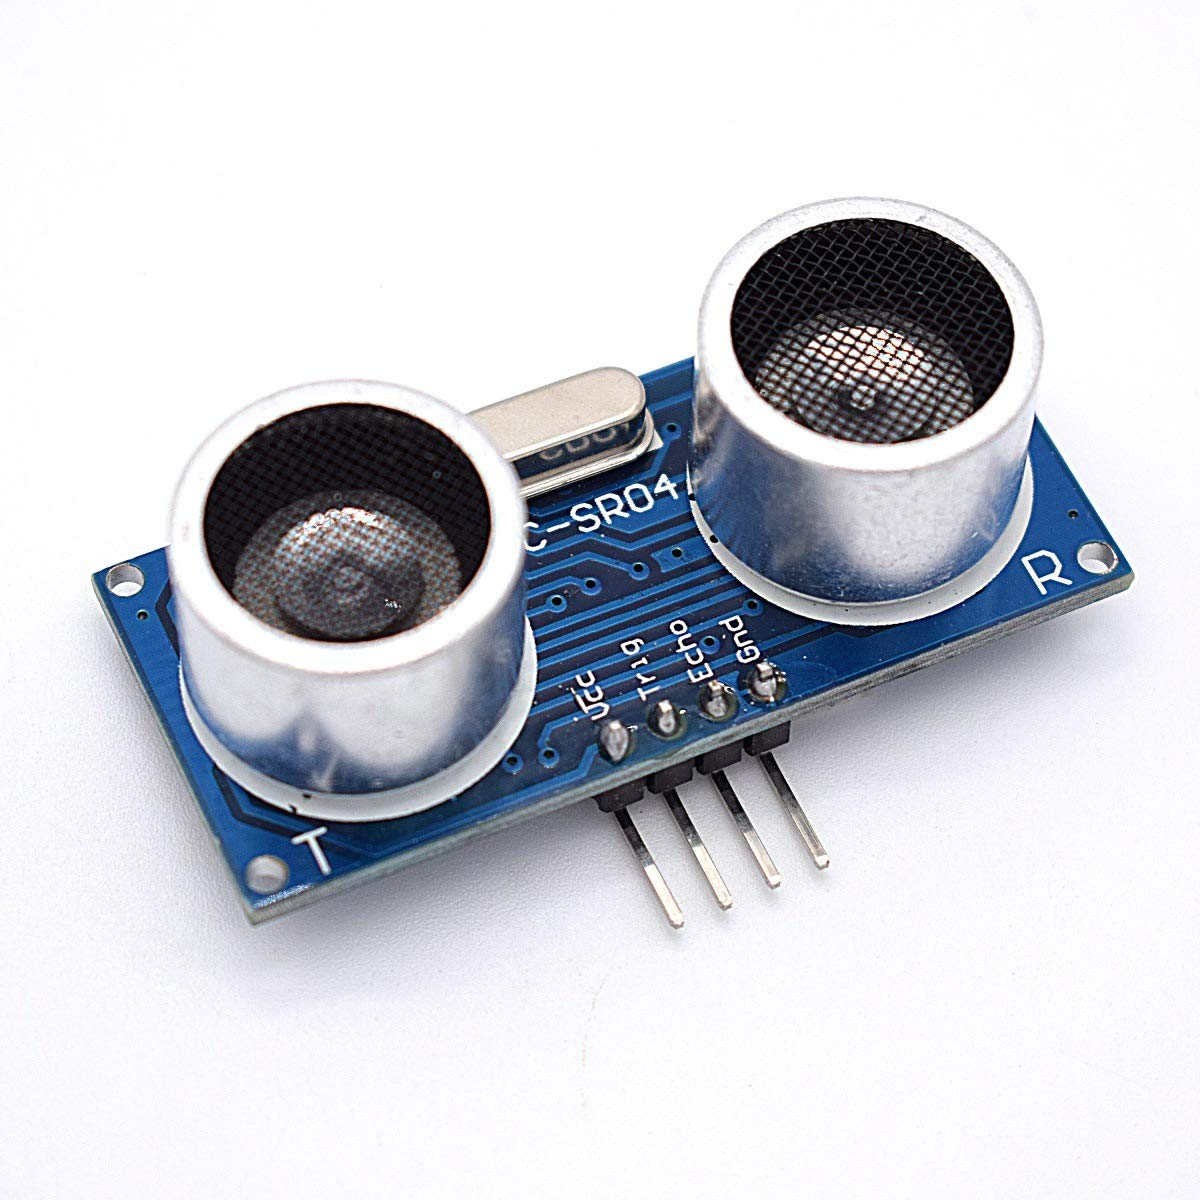
\includegraphics[width=0.4\linewidth]{Ultrasonic.jpg}
\caption{Ultrasonic Sensor (HC‑SR04) Module}
\label{fig:ultrasonic}
\end{figure}

\subsection{Buzzer Connection}
\begin{table}[!ht]
\centering
\caption{Buzzer to ESP32 Connection}
\begin{tabular}{|c|c|}
\hline
\textbf{Buzzer Pin} & \textbf{ESP32 Pin} \\
\hline
VCC    & 3.3V \\
GND    & GND \\
Signal & GPIO 13 \\
\hline
\end{tabular}
\end{table}

\section{Software Setup}
\subsection{Voice Control via Android App}
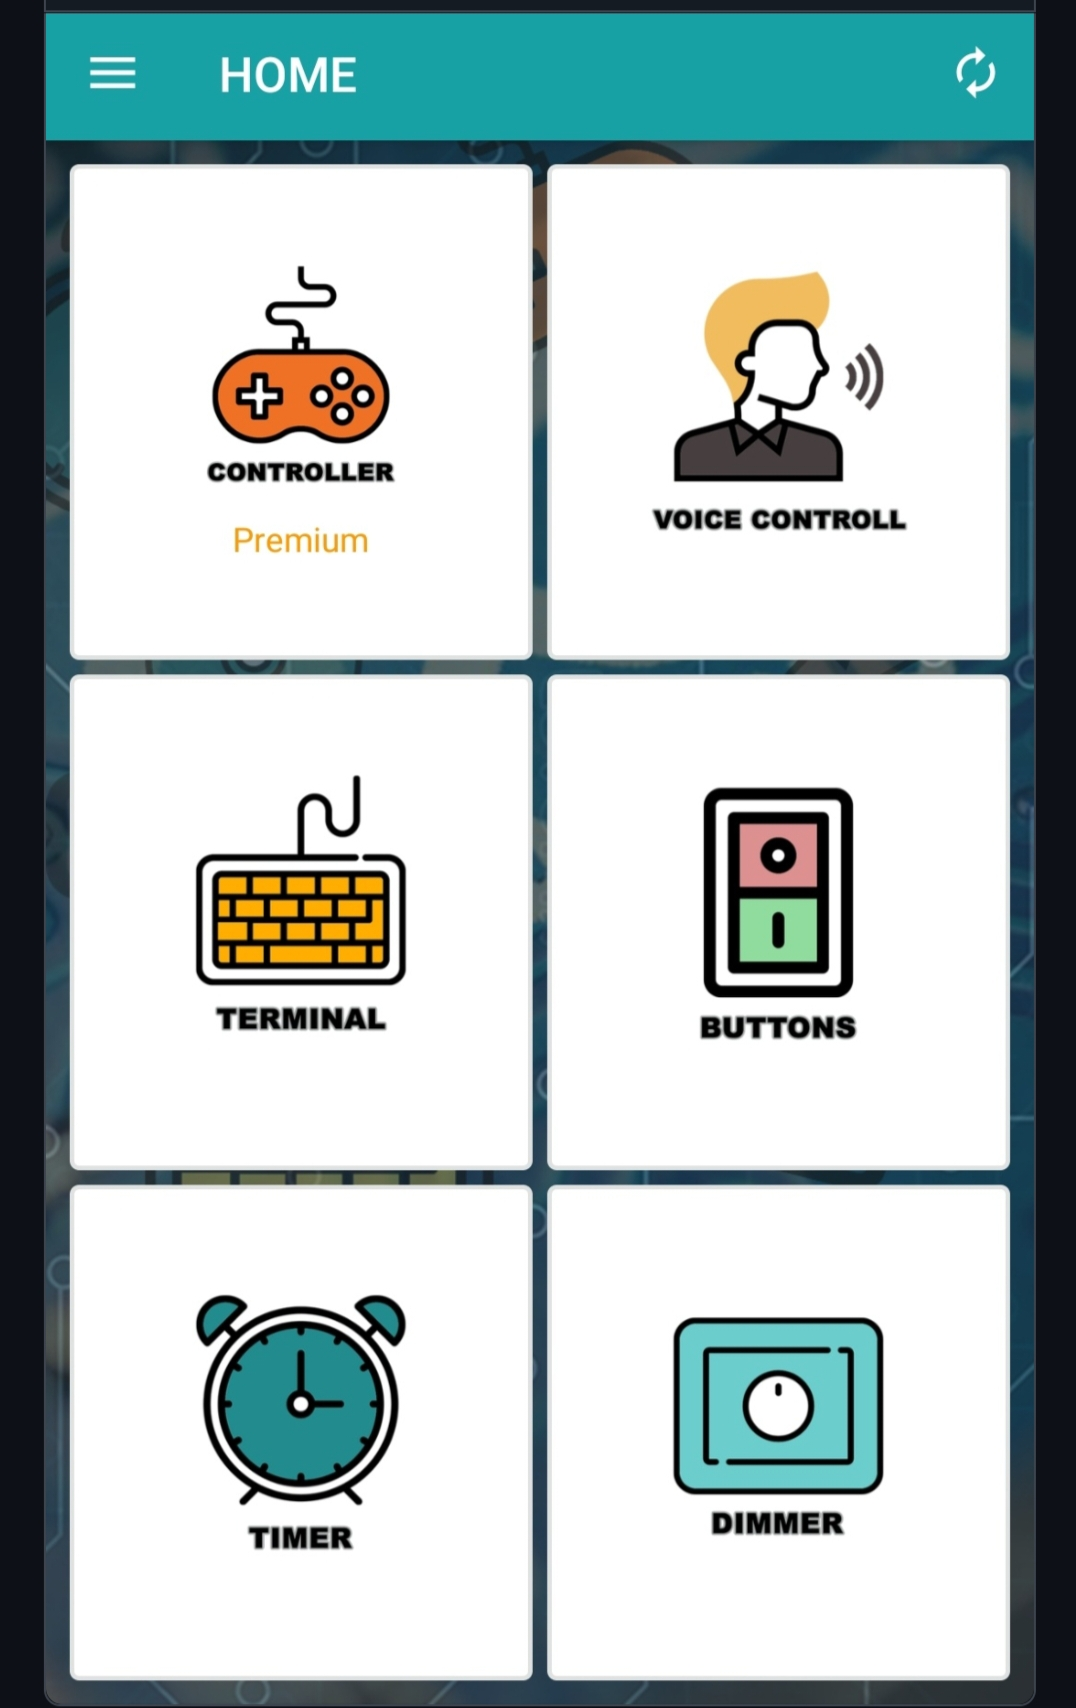
\includegraphics[width=0.4\linewidth]{Arduino_Bluetooth.jpg}
\begin{enumerate}
    \item Install the \textbf{Arduino Bluetooth Controller} app from the Google Play Store.
    \item Upload the voice‑control code tothe ESP32 using PlatformIO.
    \item Create a new PlatformIO project, select the board and framework, and replace the contents in \texttt{src/main.cpp} with the downloaded code.
    \item Power the ESP32 via a power bank and establish a Bluetooth connection from the mobile app.
    \item Use the voice control section to issue commands: \texttt{Forward}, \texttt{Back}, \texttt{Left}, \texttt{Right}, \texttt{Stop}.
    \item The UGV moves accordingly. If the ultrasonic sensor detects an obstacle within a threshold distance, the buzzer will alert and the vehicle can pause or change direction.
\end{enumerate}

\section{Conclusion and Future Work}
We have implemented a voice‑controlled UGV using the ESP32 microcontroller and L298N motor driver, enhanced with an ultrasonic sensor for obstacle detection and a buzzer for user alerting. This low‑cost prototype is ideal for academic demonstrations and rapid AI prototyping in robotics.

Future work may include:
\begin{itemize}
    \item On‑board offline speech recognition (e.g., using TensorFlow Lite) to remove dependency on cloud services.
    \item Advanced obstacle‑avoidance algorithms (e.g., using multiple sensors or vision modules).
    \item Integration of a camera or GPS module for smart navigation and environment mapping.
\end{itemize}

\begin{thebibliography}{1}
\bibitem{li2017speech}
X. Li, “Speech controlled mobile robots,” \textit{IEEE International Conference on Robotics}, 2017.

\bibitem{prasad2013voice}
R. Prasad, “Voice Controlled Intelligent Wheelchair,” \textit{IJIRCCE}, 2013.
\bibitem{esp32}
Espressif Systems, "ESP32 Series Datasheet", 2022. [Online]. Available: \url{https://www.espressif.com/sites/default/files/documentation/esp32_datasheet_en.pdf}

\bibitem{hc_sr04}
MicroElectronic, "HC-SR04 Ultrasonic Sensor Datasheet", [Online]. Available: \url{https://cdn.sparkfun.com/datasheets/Sensors/Proximity/HCSR04.pdf}

\bibitem{l298n}
STMicroelectronics, "L298N Dual Full-Bridge Driver", Datasheet, [Online]. Available: \url{https://www.st.com/resource/en/datasheet/l298.pdf}

\bibitem{bluetoothcontrol}
S. Sharma and P. Jain, "Bluetooth Controlled Robot Using Android Mobile," \textit{International Journal of Advanced Research in Computer Engineering \& Technology (IJARCET)}, vol. 4, no. 5, 2015.

\bibitem{embedded_systems}
M. Barr and A. Massa, \textit{Programming Embedded Systems}, 2nd ed., O’Reilly Media, 2006.

\bibitem{arduino_voice_control}
A. Ali, "Arduino Based Voice Controlled Robot Using Android," \textit{International Journal of Scientific \& Engineering Research}, vol. 8, no. 5, 2017.

\bibitem{speech_ai}
G. Hinton et al., "Deep Neural Networks for Acoustic Modeling in Speech Recognition," \textit{IEEE Signal Processing Magazine}, vol. 29, no. 6, pp. 82–97, 2012.

\bibitem{robotics_book}
B. Siciliano and O. Khatib, \textit{Springer Handbook of Robotics}, Springer, 2nd ed., 2016.
\end{thebibliography}

\end{document}
